\section{Resultados en Xschem, con los parámetros obtenidos del amplificador tipo \textit{cascode} \label{sec:s2}}

\begin{center}
	\begin{minipage}{12cm}
		\begin{tcolorbox}[title=Actividad 2]
			Utilizando el simulador NGSPICE en la herramienta de Xschem, simular el amplificador operacional \textit{cascode} con las razones $\frac{W}{L}$ calculadas previamente.
		\end{tcolorbox}	
	\end{minipage}
\end{center}

\begin{equation*}
	\begin{array}{l l}
		\textbf{Resultados obtenidos de la simulación} \\
		A_{V} = \frac{A_{V}(0)}{R \times C} = \frac{ 20.208314 }{ 100000.0 \times 1.2e-08 } \\
		A_{V} =  16840.261667  \\
		P_{diss} = V_{DD} \times (I_{9}+I_{10}) =  1.8 \times ( 0.0001  +  1.2e-05 ) \\
		P_{diss} =  0.2016  mW \\
		GB =  311.817097  KHz \\
		Slew Rate =  12.760688 \frac{V}{\mu s} \\
	\end{array}
\end{equation*}

\begin{figure}[ht]
	\centering
	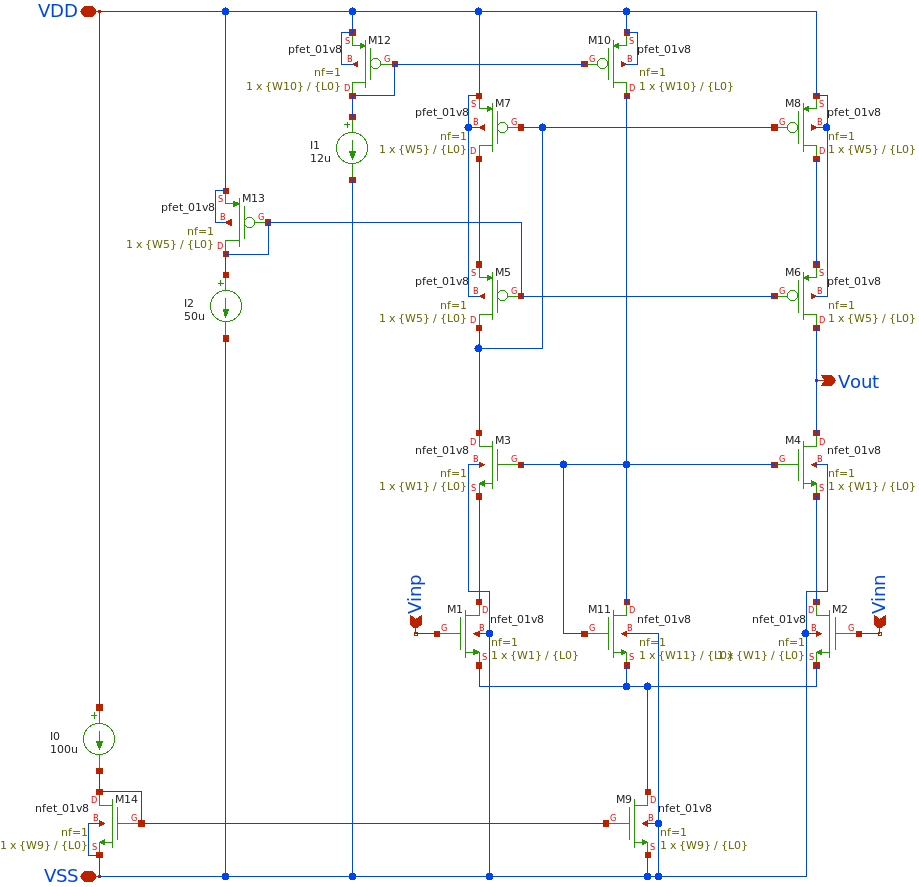
\includegraphics[scale=0.51]{CascodeOneStageOpAmp.png}
	\caption{Diagrama esquemático del amplificador operacional \textit{cascode} de una etapa. \label{fig:CascodeOneStageOpAmp}}
\end{figure}

\begin{figure}[ht]
	\centering
	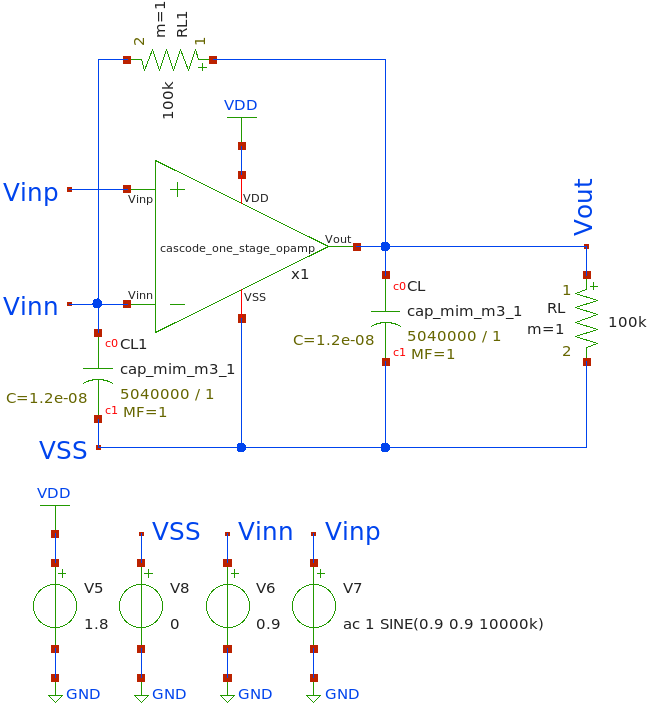
\includegraphics[scale=0.35]{CascodeOneStageOpAmpAv.png}
	\caption{Circuito utilizado para obtener la ganancia del amplificador operacional \textit{cascode} de una etapa. \label{fig:CascodeOneStageOpAmpAv}}
\end{figure}

\begin{figure}[ht]
	\centering
	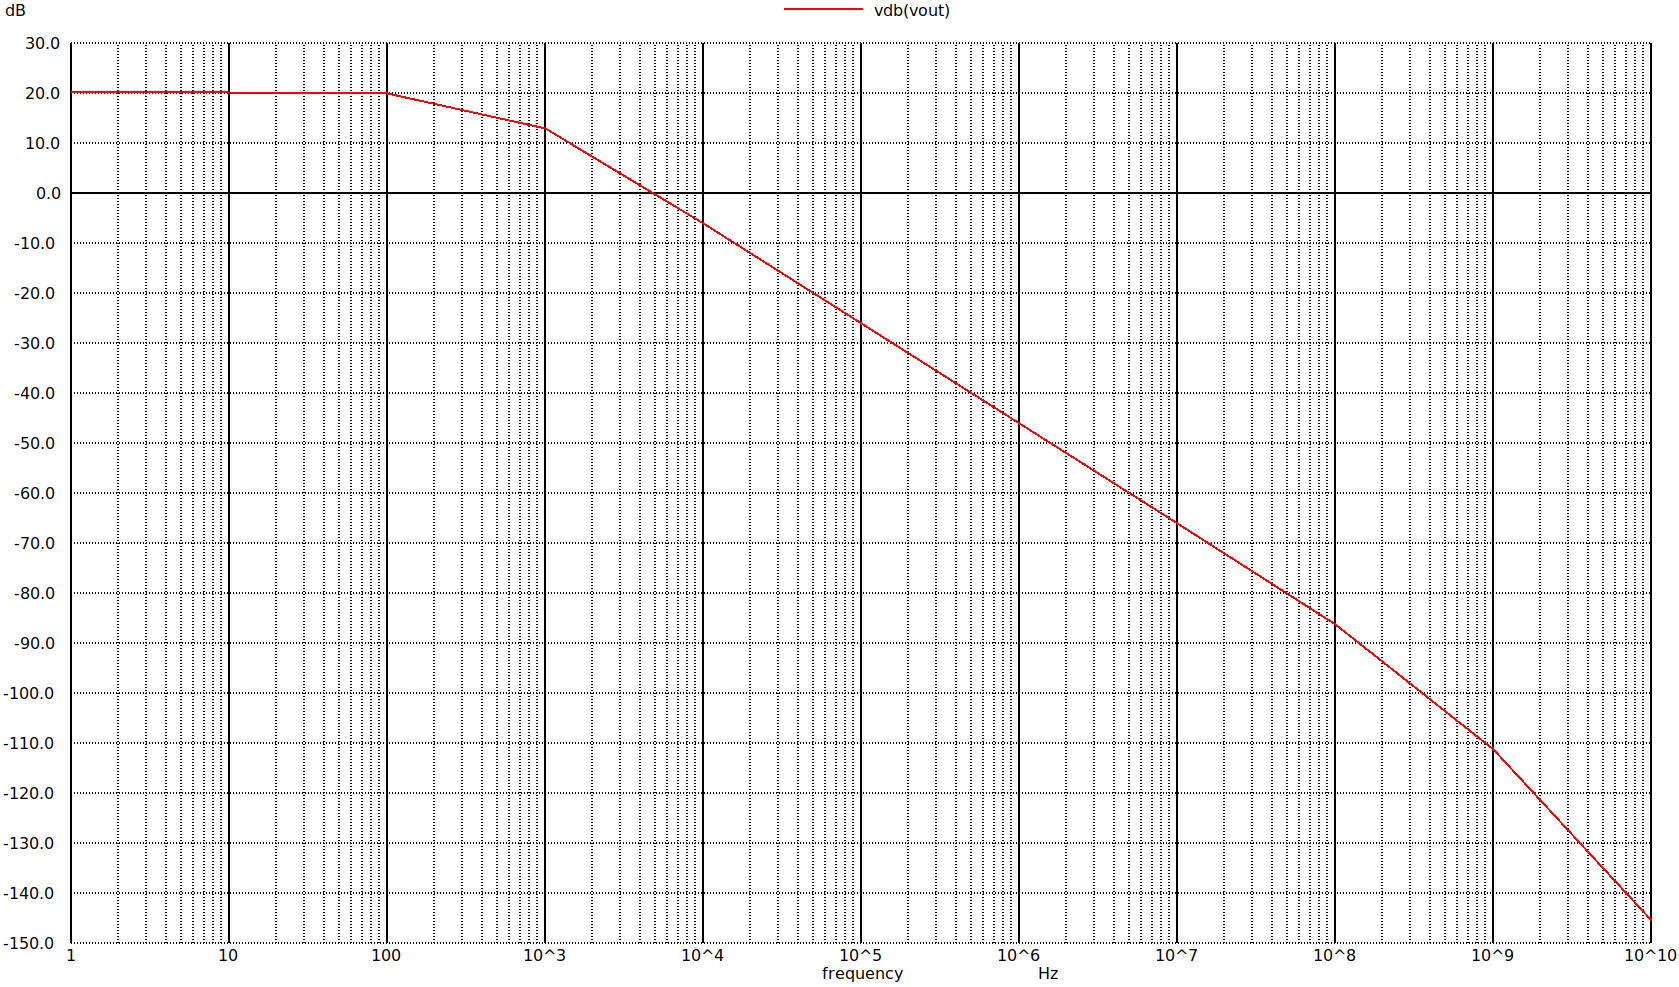
\includegraphics[scale=0.28]{CascodeOneStageOpAmpAvWF.png}
	\caption{Diagrama de Bode obtenido de la \autoref{fig:CascodeOneStageOpAmpAv}. \label{fig:CascodeOneStageOpAmpAvWF}}
\end{figure}

\begin{figure}[ht]
	\centering
	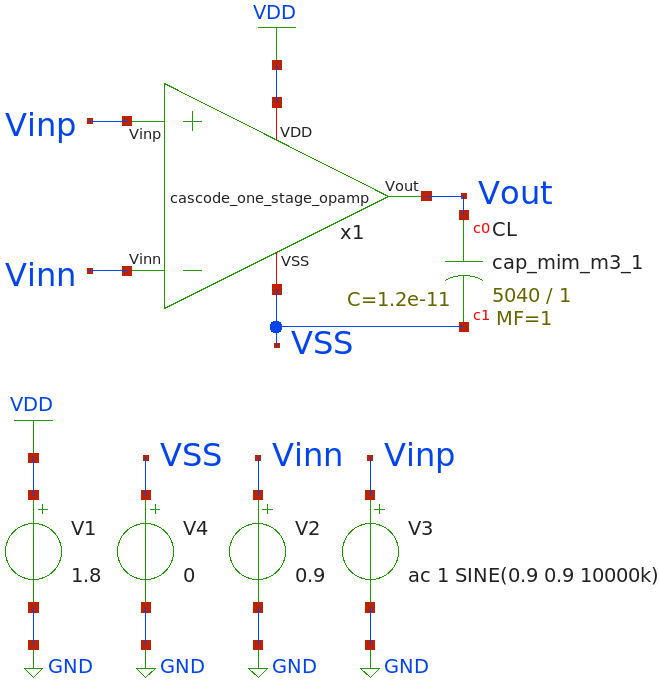
\includegraphics[scale=0.44]{CascodeOneStageOpAmpGB.png}
	\caption{Circuito utilizado para obtener la ganancia en ancho de banda (\textit{Gain Bandwidth}) del amplificador operacional \textit{cascode} de una etapa. \label{fig:CascodeOneStageOpAmpGB}}
\end{figure}

\begin{figure}[ht]
	\centering
	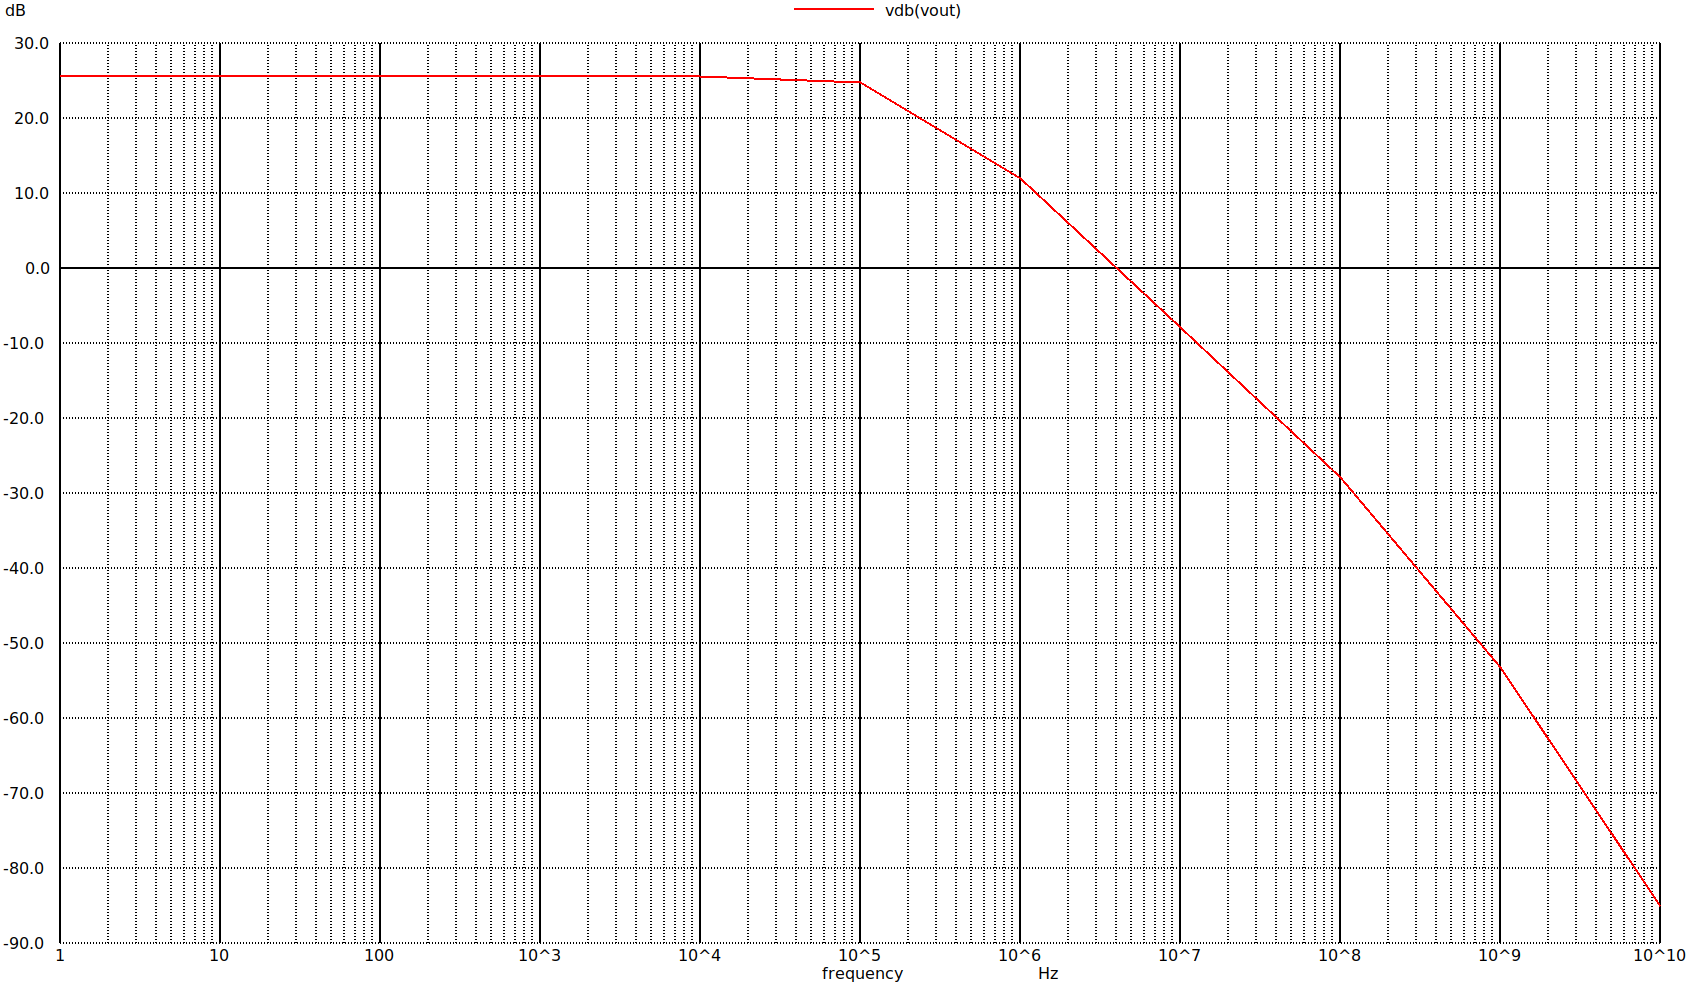
\includegraphics[scale=0.28]{CascodeOneStageOpAmpGBWF.png}
	\caption{Diagrama de Bode obtenido de la \autoref{fig:CascodeOneStageOpAmpGB}. \label{fig:CascodeOneStageOpAmpGBWF}}
\end{figure}

\begin{figure}[ht]
	\centering
	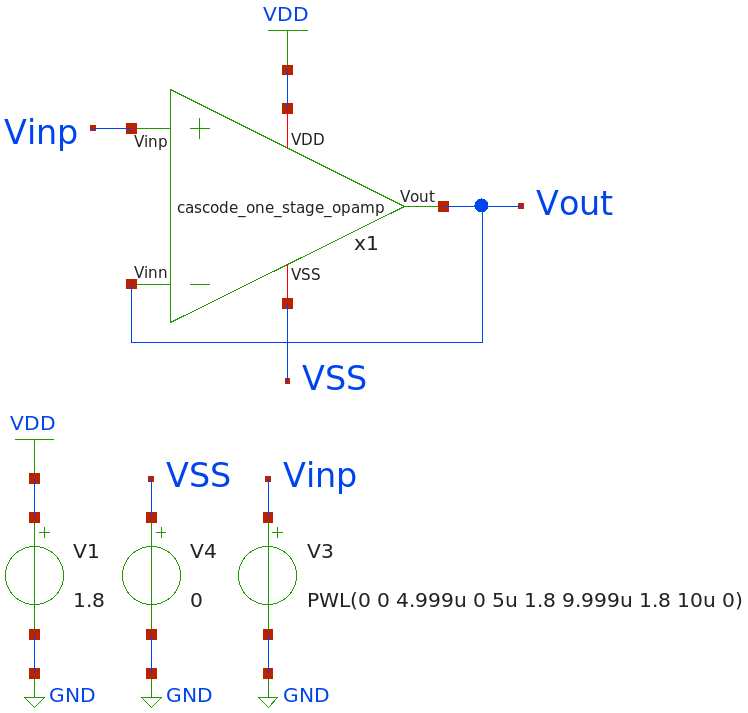
\includegraphics[scale=0.42]{CascodeOneStageOpAmpSR.png}
	\caption{Circuito utilizado para evaluar obtener el \textit{Slew Rate} del amplificador operacional \textit{cascode} de una etapa (seguidor de voltaje). \label{fig:CascodeOneStageOpAmpSR}}
\end{figure}

\begin{figure}[ht]
	\centering
	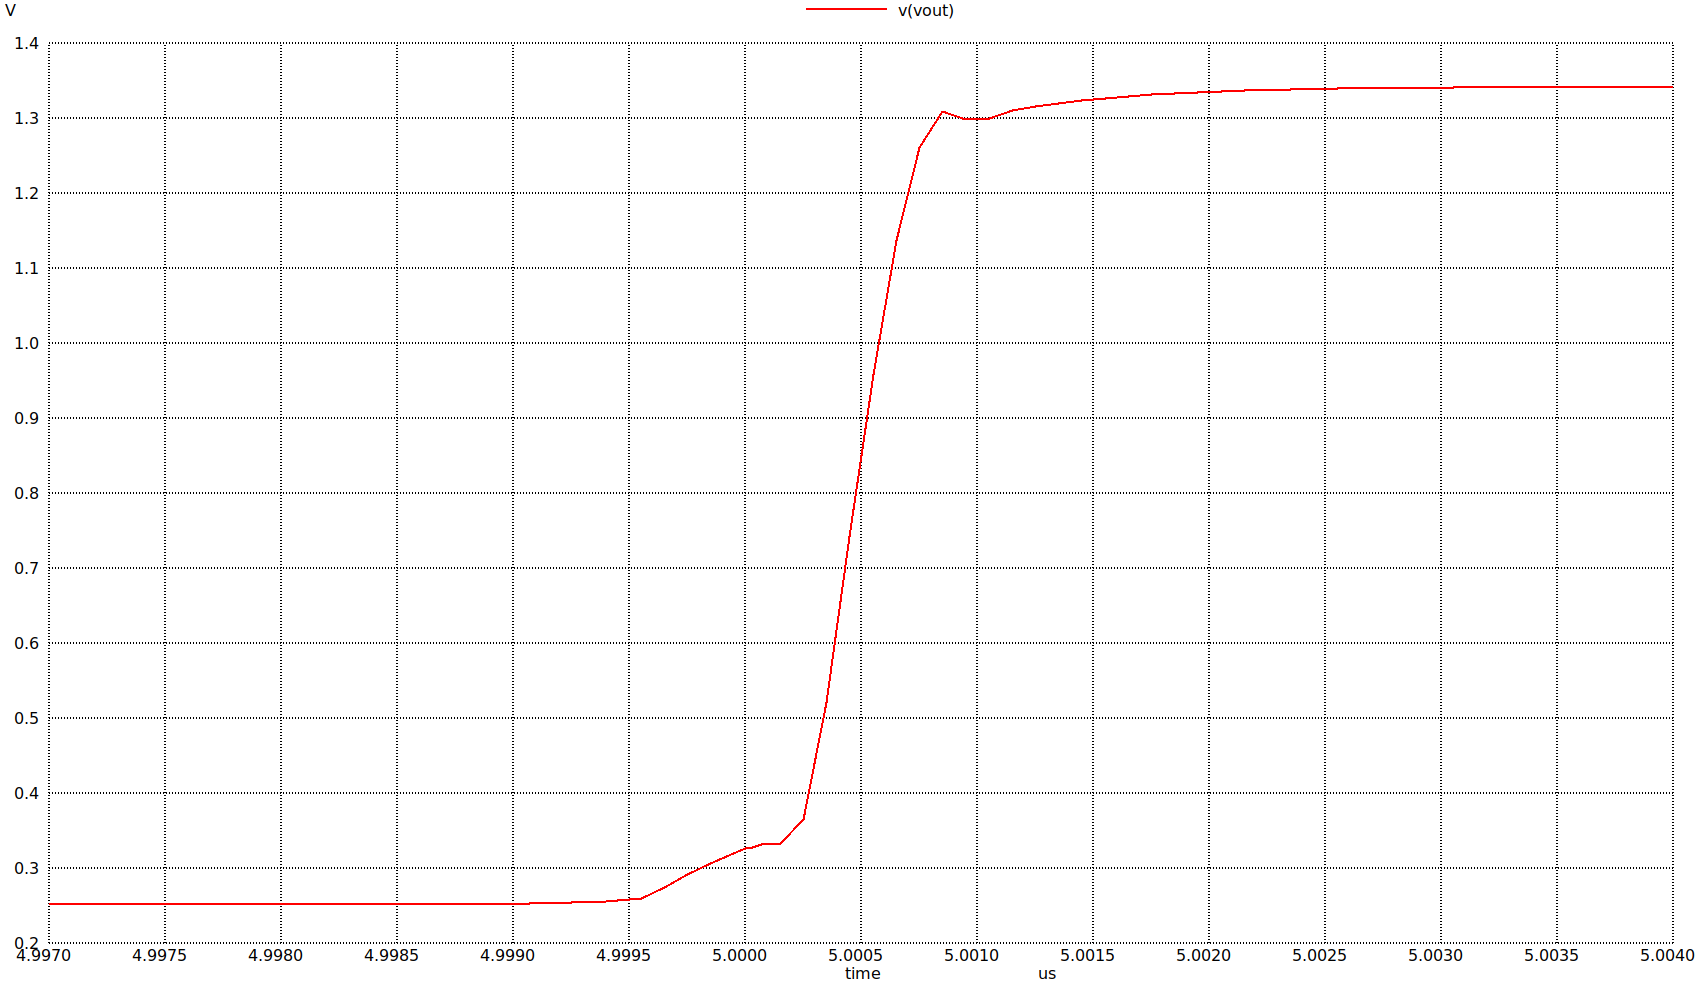
\includegraphics[scale=0.28]{CascodeOneStageOpAmpSRWF.png}
	\caption{Gráfica del voltaje de salida obtenido de la \autoref{fig:CascodeOneStageOpAmpSR}. \label{fig:CascodeOneStageOpAmpSRWF}}
\end{figure}